\chapter{Conceptual Design}

\section{Collector Analysis}

\subsection{Heat Transfer Analysis}

To model the heat transfer, depicted in Figure 3.1, occurring on the surfaces of a flat plate collector, the following simplifications can be made:

\medskip
\begin{itemize}[itemsep=3mm, parsep=-1mm]
    \item Performance is steady state. 
    \item Heat losses through the front and back are to the same ambient temperature.
    \item Construction is of the sheet and serpentine manifold type.
    \item Uniform flow exists within the tubes.
    \item Absorption of solar energy by the cover is insignificant insofar as it affects losses from the collector. 
    \item Temperature drop through the cover is negligible. 
    \item Heat flow through the cover is one-dimensional.
    \item The cover is opaque to infrared radiation. 
    \item Heat flow through the back insulation is one-dimensional. 
    \item The sky is considered a black body for long-wavelength radiation at the equivalent sky temperature.
    \item Temperature gradients around the tubes are negligible. 
    \item Properties of the collector are independent of temperature. 
    \item Dust, dirt, and snow buildup on the collector are negligible. 
    \item Shading of the collector absorber plate is negligible.
\end{itemize}

\medskip
\begin{figure}[H]
    \centering
    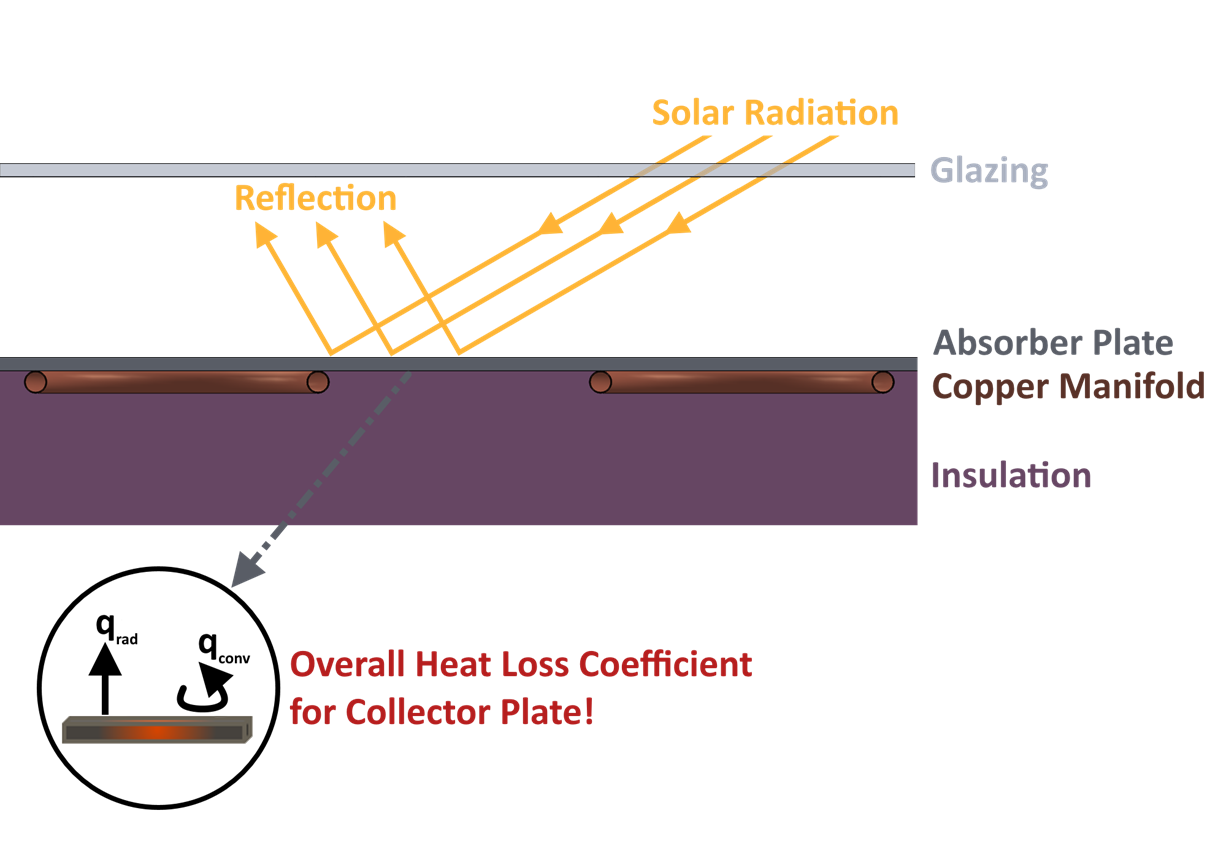
\includegraphics[width=\textwidth]{images/flat_plate_heat_transfer.png}
    \caption{Heat Transfer from a Flat Plate Collector}
\end{figure}

\medskip
The heat losses can be analytically simplified by representing the heat transfer from the collector’s absorber plate through collector’s cover at the top, and insulation at the back and subsequently, to the ambient as the thermal network depicted in Figure 3.2a. An equivalent thermal network, as shown in Figure 3.2b, can then be deduced to encompass the overall steady-state heat transfer occurring across the collector. The heat transfer analysis is derived in full detail below.

\smallskip
\begin{figure}[H]
    \centering
    \subfloat[\centering One-Cover Flat-Plate Collector] {{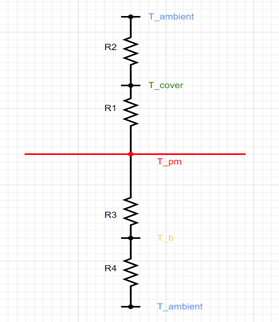
\includegraphics[width=5.2cm]{images/thermal_network.png}}}
    \qquad
    \subfloat[\centering Equivalent Thermal Network] {{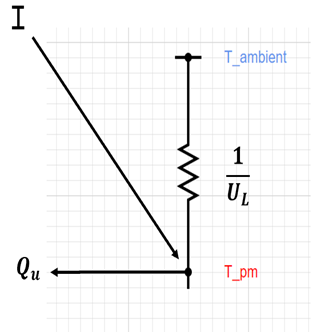
\includegraphics[width=5.2cm]{images/equivalent_thermal_network.png}}}
    \caption{Thermal Network Diagrams}
\end{figure}

\medskip
First, the top heat losses, both convective and radiative, from the absorber plate to the cover can be evaluated as follows to determine the first thermal resistance, R1:
\begin{align}
    Q_{loss, top} = h_{c, p-c}(T_{pm}-T_c) + \ddfrac{\sigma(T^4_{pm}-T^4_c)}{\frac{1}{\varepsilon_p} + \frac{1}{\varepsilon_c} - 1}
\end{align}

\begin{align}
    h_{r, p-c} = \ddfrac{\sigma(T_{pm}-T_c)(T^2_{pm}-T^2_c)}{\frac{1}{\varepsilon_p} + \frac{1}{\varepsilon_c} - 1}
\end{align}

\begin{align}
    R1 = \ddfrac{1}{h_{c, p-c} + h_{r, p-c}}
\end{align}

\bigskip
Similarly, the top heat loss, both convective and radiative, from the cover to the ambient can be evaluated as follows to determine the second thermal resistance, R2:
\begin{align}
    h_{r,c-a} = \ddfrac{\sigma\varepsilon_c (T_c + T_{sky})(T_c^2 + T_{sky}^2)(T_c - T_{sky})}{(T_c - T_a)}
\end{align}

\begin{align}
    R2 = \ddfrac{1}{h_w + h_{r,c-a}}
\end{align}

\bigskip
Finally, the total top heat loss coefficient, $U_{top}$, is found to be the inverse of the summation of R1 and R2 as follows:
\begin{align}
    U_{top} = \ddfrac{1}{R1 + R2}
\end{align}

\bigskip
A useful empirical equation for $U_{top}$ was developed by Klein (1979) following the basic procedure of Hottel and Woertz (1942) and Klein (1975). This relationship fits the graphs for $U_{top}$ for mean plate temperatures between ambient and 200\textdegree C to within $\pm 0.3 W/m^2 K$ and is represented below:
\begin{align}
    U_{top} = U_{tC} + U_{tR}
\end{align}

\newpage
The heat loss through convective effects, $U_{tC}$, can be quantified as: 
\begin{align}
    U_{tC} = \left[  \ddfrac{M}{\left(\frac{c}{T_{pm}}\right) \left( \frac{T_{pm} - T_a}{M+f} \right)^e} + \ddfrac{1}{h_w} \right]^{-1}
\end{align}

\bigskip
Where:
\begin{align}
    f   &= (1 + 0.089h_w - 0.116h_w \varepsilon_p)(1 + 0.07866N)\\
    e   &= 0.43 \left( 1 - \ddfrac{100}{T_{pm}}\right)\\
    c   &= 520 (1 - 0.000051\beta^2)\\
    h_w &= 5.7 + 3.8V_w
\end{align}

\bigskip
The heat loss through radiative effects, $U_{tR}$, can be quantified as:
\begin{align}
    U_{tR} = \ddfrac{\sigma (T_{pm}^2 + T_a^2) (T_{pm} + T_a)}{(\varepsilon_p + 0.059Mh_w)^{-1} + \frac{2M + f - 1 + 0.133\varepsilon_p}{\varepsilon_g} - M}    
\end{align}

\bigskip
Therefore:
\begin{align}
    U_{top} = \left[  \ddfrac{M}{\left(\frac{c}{T_{pm}}\right) \left( \frac{T_{pm} - T_a}{M+f} \right)^e} + \ddfrac{1}{h_w} \right]^{-1} + \ddfrac{\sigma (T_{pm}^2 + T_a^2) (T_{pm} + T_a)}{(\varepsilon_p + 0.059Mh_w)^{-1} + \frac{2M + f - 1 + 0.133\varepsilon_p}{\varepsilon_g} - M}
\end{align}

\bigskip
R3 represents the resistance to heat flow through the insulation while R4 represents the convection and radiation resistance to the environment. With appropriate back insulation, it is usually possible to assume R4 is zero and all resistance to heat flow is due to the insulation.

\medskip
The heat loss through the bottom, $U_b$, of the collector can be defined as:
\begin{align}
    U_{bottom} = \frac{1}{R} = \frac{\delta_1}{k_1}
\end{align}

\newpage
The heat loss through the sides, $U_{edge}$, of the collector can be defined as:
\begin{align}
    U_{edge} = \ddfrac{Q_{edge}}{A(T_{pm} - T_a)}
\end{align}

\medskip
Where:
\begin{align}
    Q_{edge} = A_p(T_{pm} - T_a)
\end{align}

\bigskip
The total heat loss coefficient is the sum of the heat loss coefficients for the top, bottom, and sides of the collector. It can be defined as:
\begin{align}
    U_L = U_{top} + U_{bottom} + U_{edge}
\end{align}

\begin{align}
    U_L = \left[  \ddfrac{M}{\left(\frac{c}{T_{pm}}\right) \left( \frac{T_{pm} - T_a}{M+f} \right)^e} + \ddfrac{1}{h_w} \right]^{-1} + \ddfrac{\sigma (T_{pm}^2 + T_a^2) (T_{pm} + T_a)}{(\varepsilon_p + 0.059Mh_w)^{-1} + \frac{2M + f - 1 + 0.133\varepsilon_p}{\varepsilon_g} - M}\nonumber\\
    + \frac{\delta_1}{k_1} + \ddfrac{Q_{edge}}{A(T_{pm} - T_a)}
\end{align}

\bigskip
Finally, the total useful heat gain of the collector can be quantified as:
\begin{align}
    Q_u = F'A_c\left[ I(\uptau_c \alpha_c) - U_L(T_{fi} - T_a) \right]
\end{align}

\bigskip
The fin efficiency represents the represents the efficacy with which energy absorbed by the absorber plate and the tube spacing (conceptualized as fins) is collected on the sides of the tubes for subsequent heat transfer into the working fluid:
\begin{align}
    F = \ddfrac{tanh \left[ \ddfrac{m(W-D)}{2}\right]}{\left[ \ddfrac{m(W-D}{2}\right]}
\end{align}

\newpage
Where:
\begin{align}
    m = \sqrt{\ddfrac{U_L}{k_p\delta_p}}
\end{align}

\bigskip
Physically, $F'$, the collector efficiency factor, represents the ratio of the actual useful energy gain to the useful gain that would result if the collector absorbing surface had been at the local fluid temperature. It is essentially a constant for any collector design and fluid flow rate.
\begin{align}
    F' = \ddfrac{\frac{1}{U_L}}{W\left[ \frac{1}{U_L (D + (W-D)F)} \right] + \frac{1}{C_b} + \frac{1}{\pi D_i h_{fi}}}
\end{align}

\bigskip
The collector heat removal factor is a quantity that relate the actual useful energy gain of the collector to the useful energy gain has the entire collector surface were at the fluid inlet temperature. 
\begin{align}
    FR = \ddfrac{mC_p}{A_c U_L}\left[ 1-\exp\left( \frac{-A_c U_L F'}{mC_p}\right)\right]
\end{align}

\bigskip
It’s important to note that, as the mass flow rate through the collector increases, the temperature rise through the collector decreases. This corresponds to lower losses as the average collector temperature is lower, leading to an increase in the useful energy gain. This increase is reflected by an increase in the collector heat removal factor $FR$ when the mass flow rate increases.

\subsection{Collector Efficiency}

The collector’s instantaneous efficiency is defined as the ratio of useful heat energy gain to total energy incident on the collector’s surface:
\begin{align}
    \eta = \frac{Q_u}{I A_c}
\end{align}

\bigskip
The day-long collector efficiency is the summation of instantaneous efficiencies at known time steps, in our case, on an hourly basis:
\begin{align}
    \eta_{day} = \frac{\sum Q_u}{\sum I A_c}
\end{align}

\bigskip
As seen in the equations above, the absorber plate’s mean temperature is important in determining the values evaluated by the previous governing equations. With many unknowns, this value can only be determined through an iterative solution approach using an initial guess for the plate mean’s temperature. For our purposes, an initial guess of $T_{pm} = T_{fi} + 5$ is reasonable [33]. Following the iterative algorithm described in the 'Code Logic' below, and summarized in Figure 3.4, the equation below can be used to determine a convergent solution for the final mean temperature of the plate:
\begin{align}
    T_{pm} = T_{fi} + \ddfrac{\frac{Q_u}{A_c}}{FRU_L} (1 - FR)
\end{align}

\subsection{Thermodynamic Cycle Analysis \& Collector Efficiency Optimization}

In thermodynamics, heat pump cycles are bound by two reservoir temperatures, namely, the evaporation and the condensation temperatures. For the purposes of the system, the condensation temperature is regarded as a set point: since the system is designed to support an outlet water temperature of 55\textdegree C for domestic use, $T_{cond}$ is constrained to be approximately 60\textdegree C. Determining the optimal, steady state evaporation temperature on which to base the collector design is key, not only to optimizing the flat plate collector’s area, but also to minimizing the radiative and convective heat losses emanating from its surfaces. Closely tied to the ambient temperatures, the evaporation temperatures of the working fluid circulating within the collector’s manifold dictate the useful heat gain of the collector or, more specifically, the efficiency of the collector, and correspondingly, the $COP$ of the overall system. Referring to ASHRAE’s heat pump \& air conditioning design conditions for Calgary, an initial range of design evaporation temperatures between -10\textdegree C and 10\textdegree C was selected.

\medskip
Additionally, meteorological data sets encapsulating average, hourly, winter-day temperatures and Irradiance values were loaded into the MATLAB [36] file. Using a C++ Fluid Properties’, MATLAB-accessible library, CoolProp [18], the thermodynamic states of the Refrigerant R410A, including temperatures, pressures, enthalpy, and entropy, were determined for points 1 through 4 of the thermodynamic cycle. As depicted in Figure 3.3, the isobar between on which states 2-3 lie represents the set, saturation pressure corresponding to the design condensation temperature of 60\textdegree C. The collection of dashed isobars on which states 4-1 lie correspond to the saturation pressures of the chosen range of evaporation temperatures to undergo analysis. To simplify the analysis, the following assumptions of the thermodynamic cycle were made:

\newpage
\begin{enumerate}[itemsep=3mm, parsep=-1mm, label=\roman*.]
    \item Constant pressure heat addition occurs in the collector.
    \item Constant pressure heat rejection occurs in the condenser.
    \item Isentropic compression occurs between states 1-2 in the compressor.
    \item Isenthalpic expansion occurs between states 3-4 in the expansion valve.
    \item The refrigerant enters the compressor at a quality of 1 or in a saturated vapor state.
\end{enumerate}

\medskip
These assumptions will later be corrected for thorough accounting for sub-component efficiencies as well as pressure drop in the collector.

\medskip
\begin{figure}[H]
    \centering
    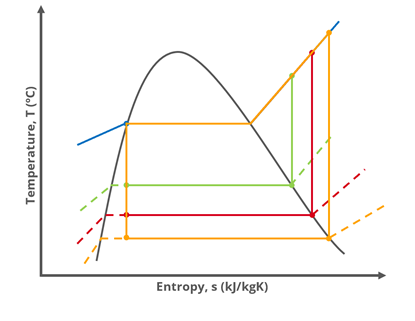
\includegraphics[width=9.5cm]{images/ts_diagram.png}
    \caption{T-s Diagram for Probable Design Evaporation Temperatures}
\end{figure}

\medskip
Using CoolProp [18], the team determined the performance parameters of the isolated heat pump cycle, namely, $Q_L$, $Q_H$, $W_{comp}$ and $COP$. With $W_{comp}$  or theoretical compressor work in mind, appropriate sizing for the compressor was determined. Next, code was developed which amalgamated the flat plate collector’s governing equations and, through iteration, allowed for the determination of the flat plate’s mean temperature. Figure 3.4 below depicts the complete iteration algorithm utilized in the MATLAB code.

\medskip
\begin{figure}[H]
    \centering
    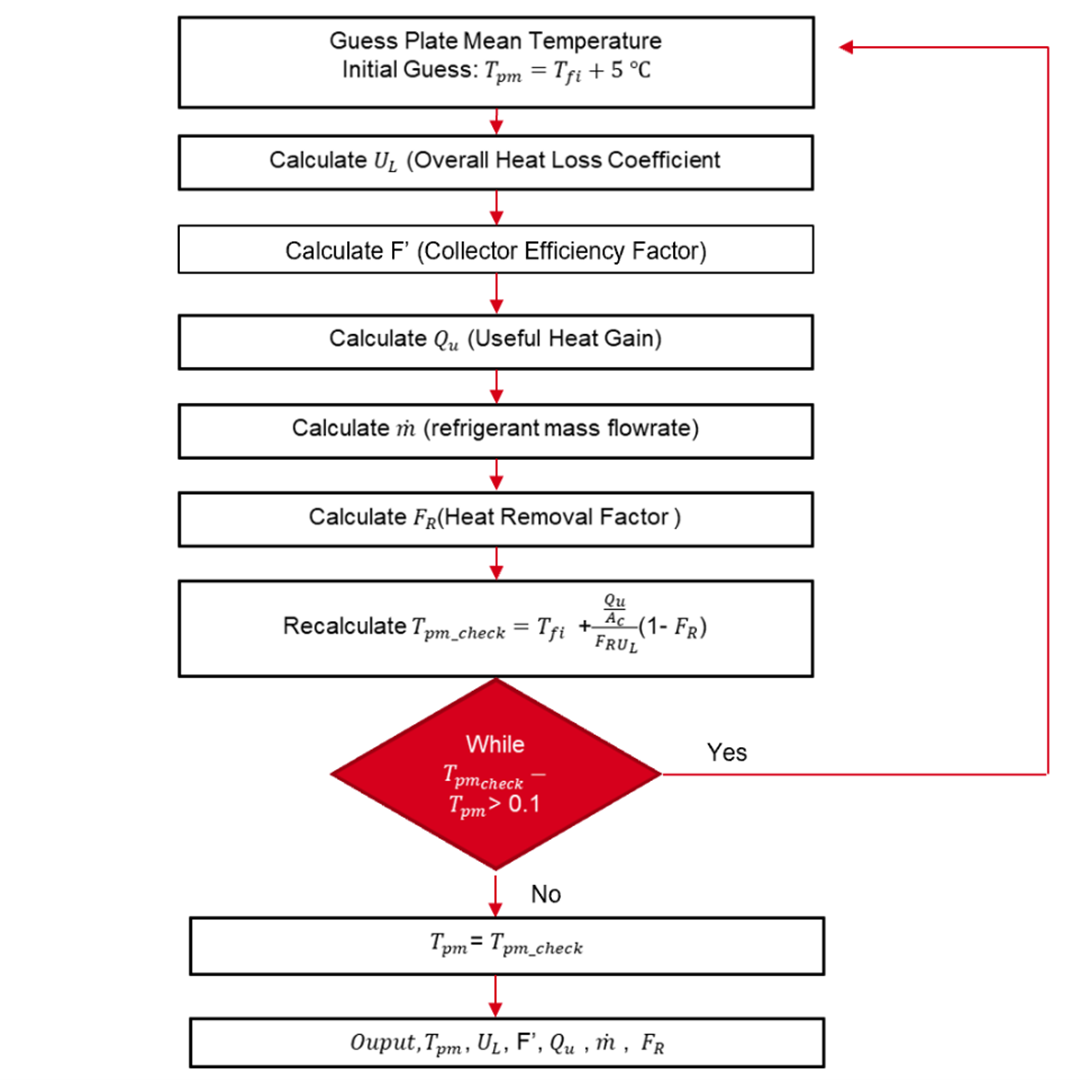
\includegraphics[width=12cm]{images/iterative_solution.png}
    \caption{Iterative Solution for Flat Plate Mean Temperature}
\end{figure}

\medskip
Once the flat plate’s mean temperature was determined, the collector’s useful heat gain, and, subsequently, the collector’s efficiency was evaluated for every data point in the evaporation temperature range. The evaporation temperature’s impact on the isolated heat pump cycle $COP$ is diametrically opposed to its impact on the useful heat gain of the collector: on one hand, the $COP$ of the heat pump cycle increases as the gap between the evaporation and condensation reservoir temperature is minimized, or when the chosen evaporation design temperature is elevated. On the other hand, the collector’s efficiency declines with the elevation of evaporation temperature as a result of increased heat losses from its surfaces. Noting this inverse relationship, it’s deducible that a plot of the product of $COP$ and Collector Efficiency (a quantity defined as the overall system $COP$) versus evaporation temperature would exhibit a characteristic inflection point at the evaporation temperature that maximizes both these inversely related parameters. For the DX-SAHP, the inflection point was seen to occur at -2\textdegree C. Knowing the design evaporation temperature, the team was able to subsequently determine the predicted collector efficiency, and the predicted useful, net collected heat. These values will later be leveraged to evaluate the theoretical performance of the DX-SAHP against the logged experimental performance. Using the code, the team also determined the system’s necessary flow rate, which supplemented the selection process of the remaining sub-components of the heat pump cycle.

\section{Collector Final Design}

\subsection{Insulation Selection}

Insulation is one of the most efficient ways to save energy by reducing heat loss during winter and thus lowering energy bills [36]. Reducing heat loss in the collector means the compressor will have to do less work to meet the hot water requirements. For the flat plate collector, it was essential to investigate the concepts pertaining to location of any heat losses to the surroundings, type, thickness, and cost of insulation.

\medskip
In the solar flat plate collector, heat losses occur through the absorber plate by top losses. As the plate heats up, some of this heat is then transferred to R-410A (within the copper tubing of the collector that is brazed beneath and to the aluminum absorber plate), while some of the heat being lost to its surroundings. The heat losses occurring through the back, and sides of the collector are respectively known as bottom and edge losses [36]. From heat transfer and thermodynamic contexts, it is understood that these heat losses occur in the form of conduction, convection, and radiation [36].

\medskip
Based on the engineering analysis and design of the collector, the bottom and sides require insulation as to minimize any heat losses and the consideration of an insulation cover being required in case of probable exposure area that is responsible for the occurrence of any heat losses.

\medskip
The insulation materials representative of some of the materials commonly used in solar flat plate collectors and in the industry are as follows:

\medskip
\begin{itemize}[itemsep=3mm, parsep=-1mm]
    \item Fiberglass wool. 
    \item Rigid polyurethane foam.
    \item Mineral wool.
    \item Expanded polystyrene.
    \item Extruded polystyrene.
\end{itemize}

\newpage
The following table represents the range of thermal conductivity values, temperature, and R-values [37] for the mentioned types of insulation materials.

\medskip
\begin{table}[H]
\centering
\caption{Range for Thermal Conductivity, Temperature, and R-Value for Insulation}
\rowcolors{2}{gray!20}{white}
\begin{tabular}{|P{40mm}|P{35mm}|P{35mm}|P{35mm}|}
    \hline
    \rowcolor{orangeRed}
    Insulation Type & Thermal Conductivity, k $[W/mK]$ & Temperature Range & R Value [per inch of thickness] \\
    \hline
    Fiberglass Wool         & 0.023 - 0.040 & -195\textdegree C to 230\textdegree C & R-3.7 to R-4.2  \\
    Rigid Polyurethane Foam & 0.020 - 0.035 & 62\textdegree C to 93\textdegree C    & R-3.4 to R-6.7 \\
    Mineral Wool            & 0.033 - 0.040 & Maximum: 649\textdegree C             & R-3.7 to R-4.3 \\
    Expanded Polystyrene    & 0.030 - 0.040 & Maximum: 75\textdegree C              & R-3.9 to R-4.7 \\
    Extruded Polystyrene    & 0.025 - 0.040 & Maximum: 74\textdegree C              & R-5.0 to R-5.6 \\
    \hline
\end{tabular}
\end{table}

\medskip
The following table identifies the American Society for Testing and Materials (ASTM) specification, material type, and/or grade for some of the insulation materials that are commonly used in the industry [38].

\medskip
\begin{table}[H]
\centering
\caption{Common Types of Insulation - Based on ASTM}
\rowcolors{2}{gray!20}{white}
\begin{tabular}{|P{50mm}|P{50mm}|}
    \hline
    \rowcolor{orangeRed}
    Material & Insulation Standard \\
    \hline
    Cellular Glass   & ASTM C 552 Type II        \\
    Elastomeric      & ASTM C 534 Type I, Gr 1   \\
    Fiberglass       & ASTM C 547 Type I         \\
    Flexible Aerogel & ASTM C 1728 Type I, Gr 1B \\
    Phenolic         & ASTM C 1126 Type III      \\
    Polyethylene     & ASTM C 1427 Type I, Gr1   \\
    Polyisocyanurate & ASTM C 591 Type IV        \\
    Polystyrene      & ASTM C 578 Type XIII      \\
    \hline
\end{tabular}
\end{table}

\medskip
Based on the above analysis, mineral wool was selected as the insulating material to be used for the solar flat plate collector due to its excellent thermal properties. Mineral wool has low thermal conductivity values, allowing for less heat to be passed through and lost to the surroundings. The suitable temperature range allows for use up to 649\textdegree C as this material will not melt until temperatures reach beyond 1,000\textdegree C. The R-values are within a range of R-3.7-R-4.3, allowing for it to suitably resist heat flow. In addition, mineral wool is naturally moisture resistant [39].

\newpage
\subsection{Glazing Selection}

Glazing refers to the top cover of the solar collector. It has three main purposes:

\medskip
\begin{enumerate}[itemsep=3mm, parsep=-1mm, label=\roman*.]
    \item Protect the internal components from the outside environment.
    \item Minimize heat loss due to convection and radiation from the absorber plate.
    \item Allow as much solar radiation through as possible.
\end{enumerate}

\medskip
The two main materials used for solar collector glazing are glass and polycarbonate.

\medskip
The main parameter to consider when choosing the glazing is the transmittance. Transmissivity is a measure of how much light passes through the object for a given wavelength. For a solar collector, the glazing should let through as much sunlight as possible but be opaque to the infrared radiation emitted by the absorber plate. This will allow for the most heat gain possible. The secondary parameters which should be minimized are the absorptance and reflectance of the glazing. The absorptivity is a measure of how much radiation is absorbed for a given wavelength and reflectivity is how much is reflected [40].

\medskip
Another important factor to consider is the solar heat gain coefficient (SHGC). The SHGC is a measure of how much solar radiation is admitted. A high SHGC rating indicates that the materials are more effective at collecting solar heat, which is better for a solar collector [41].

\medskip
\begin{table}[H]
\centering
\caption{Properties of Various Glazing Materials}
\rowcolors{2}{gray!20}{white}
\begin{tabular}{|P{31mm}|P{23mm}|P{23mm}|P{10mm}|P{34mm}|P{17mm}|}
    \hline
    \rowcolor{orangeRed}
    Glazing Type & Temperature Range & Transmissivity & SHGC [42][43] & Thermal Expansion Coefficient $(in/in/F)$ & Density $(kg/m^3)$ \\
    \hline
    Low Iron Tempered Glass [44]  & -50\textdegree C to 240\textdegree C & 91.5\% & $\sim 0.91$ & 4.9E-6  & 2530 \\
    Polycarbonate (Standard) [45] & -50\textdegree C to 120\textdegree C & 86\%   & $\sim 0.80$ & 3.75E-5 & 1197 \\
    Sun-Lite [46]                 & -50\textdegree C to 120\textdegree C & 86\%   & $\sim 0.80$ & 3.6E-5  & 1200 \\
    Lexan 9034 [47]               & -40\textdegree C to 100\textdegree C & 88\%   & $\sim 0.80$ & 3.75E-5 & 1197 \\
    SunTuf [48]                   & -40\textdegree C to 100\textdegree C & 90\%   & $\sim 0.80$ & 3.6E-5  & 1200 \\
    \hline
\end{tabular}
\end{table}

\medskip
As seen from Table 4 above, all the materials found met the temperature requirement of -30\textdegree C to 30\textdegree C. Low iron tempered glass was found to have the highest transmissivity, highest solar heat gain coefficient, and lowest coefficient of thermal expansion. Glass was found to be more opaque to the long wave radiation emitted by the absorber plate, and therefore better at trapping heat [49]. Whereas polycarbonate was found to transmit more IR radiation [50]. Additionally, polycarbonate will yellow over time from exposure to UV rays [51]; this will reduce the amount of light transmitted by it. However, glass is more than two times heavier than the polycarbonate sheets and more prone to breaking. So extra care will need to be taken when installing it in the collector.

\subsection{Plate Material Selection}

The absorber plate is the component which absorbs solar radiation and emits it as infrared radiation. This heat is then absorbed by the copper piping and then the refrigerant. For this purpose, the plate must have high absorptivity, heat conductivity, and emissivity. The most common materials for the absorber plate are copper, aluminum, and steel; the thermal conductivities of these metals are $398 W/mK$, $247 W/mK$, and $45 W/mK$ respectively [52] [53]. Steel was found to have too low thermal conductivity for this application. The price of copper was \$9.55/kg [54] and aluminum was \$6.33/kg [55]. Aluminum was selected for our application because it was more readily available.

\medskip
A selective coating will be applied to the absorber plate to increase the amount of sunlight absorbed. The coating should have high absorbance and low emissivity, so all the absorbed heat will be transferred to the aluminum plate. It should also be able to withstand high temperatures and be UV resistant. Thurmalox 250 was identified as a coating specifically suited for solar thermal collector application [56].

\subsection{Manifold Design}

To determine the copper tube design beneath the absorber plate of the solar flat plate collector, it was convenient to create a two-dimensional drawing to determine the layout. The design of the tubing helped determine the overall length of tubing that would be required. A serpentine tube design was selected as it maximizes the amount of surface area, and for R-410A, for heat transfer to occur within a limited amount of space [57].

\medskip
The serpentine copper tube design for the flat plate collector was completed based upon the following criteria:

\medskip
\begin{enumerate}[itemsep=3mm, parsep=-1mm, label=\roman*.]
    \item Tube pitch of 3/4 inches [19.05 mm].
    \item Tube bend diameter of 3 15/16” [100 mm].
    \item Leave 1 15/16” [50mm] on each side of absorber plate.
\end{enumerate}

\medskip
In the following figure, two designs were created, (a) and (b). Both designs have an equal manifold spacing. The design for (a) was selected as this design leads to a greater surface area allowing for more heat transfer to occur. With the design for (a) having more U-bends in the tubes, this allows for more time for heat transfer to take place with R-410A. A tube bending tool may be used to force the tube to conform to a bend diameter of 3 15/16” [100 mm]. The overall straight length between both designs differs by 5 inches [127 mm] in which the cost between both tube designs will be similar.

\newpage
\begin{figure}[ht]
    \centering
    \subfloat[\centering Horizontally Spaced Manifold] {{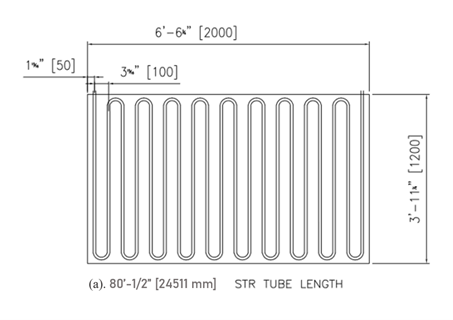
\includegraphics[width=7.7cm]{images/manifold_type_a.png}}}
    \qquad
    \subfloat[\centering Vertically Spaced Manifold] {{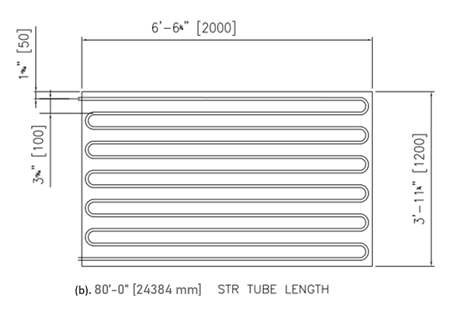
\includegraphics[width=7.7cm]{images/manifold_type_b.png}}}
    \caption{Two-Dimensional Designs of Serpentine Copper Tube Manifold}
\end{figure}

\subsection{Final Collector Model}

\begin{figure}[H]
    \centering
    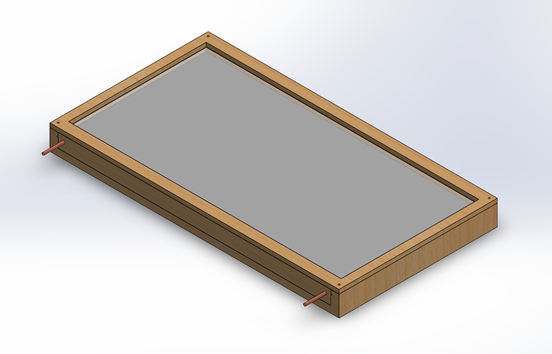
\includegraphics[width=\textwidth]{images/collector_assembly.png}
    \caption{SOLIDWORKS Assembly of Solar Thermal Collector}
\end{figure}

\begin{figure}[H]
    \centering
    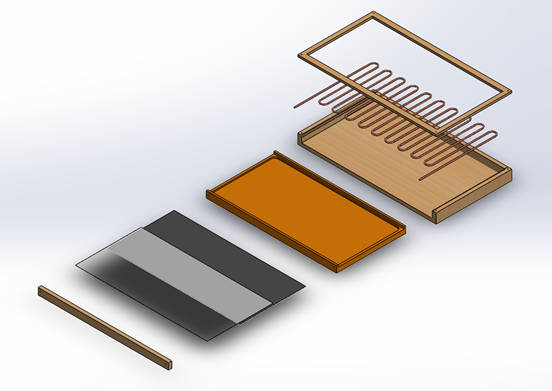
\includegraphics[width=\textwidth]{images/collector_assembly_exploded.png}
    \caption{Exploded View of Solar Thermal Collector}
\end{figure}

\medskip
Although the collector frame is a simple enclosure, sizing limits and assembly considerations must be understood. The wood casing will be created in multiple parts and grooves will be added to account for the thermal expansions of both the glass and absorber plates during winter thermal contractions and summer thermal expansions. 

\medskip
The depth of the grooves will be determined using the equation for linear thermal expansion.
\begin{align}
    \Delta L = \alpha_L L_c \Delta T
\end{align}

\medskip
The order in which the components are assembled must be taken in consideration to avoid scenarios where components are blocked by other components. As component selections become finalized and are ready to order, fitment tolerances will be subsequently added.

\newpage
\section{Final Component Selection}

For component matching, external to the solar flat plate collector, suitable components and materials for the system based on data and design parameters are being selected. The components mentioned below are the compressor, condenser, expansion valve, control system, and minor parts. The evaluation of manufacturing methods and metal-joining processes as well such as, brazing and/or welding, and use of items such as couplings, and tube adapters have been taken under consideration. The following selection of components are preliminary as of now and will be finalized in the Final Design Report.

\subsection{Compressor Selection}

A compressor is required after the collector to meet the domestic hot water requirements. A hermetically sealed compressor is ideal for domestic heat pump systems. The compressor will be a single stage, rotary vane, positive displacement compressor. The motor will be a single phase, variable speed motor. The compressor must operate within the specified voltage of approximately 110/120 V and 50-60 Hz [58]. In the case where it is greater, further in-depth investigation into transformers [59] [60] or power amplifiers is required to overcome this difference.

\medskip
The compressor selection is based on the lowest evaporating temperature of -10°C. To obtain a condensation temperature of 60\textdegree C, the pressure differential needs to be controlled via the motor speed.

\medskip
The compressor is also evaluated based on the criteria shown below:

\medskip
\begin{enumerate}[itemsep=3mm, parsep=-1mm, label=\roman*.]
    \item Compatibility with R-410A.
    \item Working pressure ratings.
    \item Lubricant compatibility.
    \item Power requirement.
\end{enumerate}

\medskip
The power requirement for the compressor was found to be 1.138 horsepower based on the required flow rate.

\medskip
The rotary vane variable speed hermetic compressor was selected for this project. These types are commonly used for appliances and for residential applications. It may be applied for the purposes of the DX-SAHP as it operates at low capacities, requiring less input power. The compressor works by rotating action of a roller inside a cylinder to compress the refrigerant.

\medskip
The following figure shows what the hermetic variable speed compressor looks like for a low input power rating. However, this compressor is not a finalized selection as vendors are currently being contacted.

\newpage
\begin{figure}[H]
    \centering
    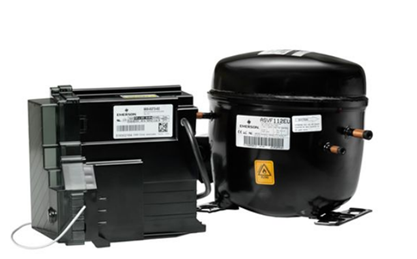
\includegraphics[width=8cm]{images/var_speed_compressor.png}
    \caption{Hermetic Variable Speed Compressor [61]}
\end{figure}

\medskip
The compatibility between the hermetic variable speed compressor and electronic expansion valve is crucial as this controls the pressure differential of R-410A through the compressor and the amount of flow rate through the valve. Vendors have been provided the design specifications, controller requirements, and refrigerant parameters to size these components. The copper piping, having a diameter of 0.75 inches, is to be connected to the suction and discharge of the compressor and valve. The determination of the diameters and materials of these lines are being communicated with the vendor as to allow the easiest route for metal-joining and installation purposes. The two choices, as of now, to connect the external piping to the suction/discharge lines of both the compressor and valve, can either be done by brazing the copper piping to the connecting tubes and/or by use of a copper adapter tube [62]. The use of an adapter tube allows for the connection of the suction/discharge connector to be connected to the external piping without the need of expanding the connectors or reducing the diameters of the connection tubes.

\subsection{Condenser Selection}

The condenser is responsible for the heat transfer between the refrigerant and the domestic hot water. It also stores and insulates the water for immediate use if required. The basic components of the condenser are a hot water tank with a copper condensing coil inside to allow for heat transfer between the refrigerant and the water. A simple heat exchanger will not suffice as hot water needs to be stored for use when there is no solar radiation available.

\medskip
The selection criteria for the condenser are as follows:

\medskip
\begin{enumerate}[itemsep=3mm, parsep=-1mm, label=\roman*.]
    \item Must be able to store at least 225L of water.
    \item Max condensing coil pressure of 3800kPa.
    \item Max condensing coil temperature of 85\textdegree C.
    \item Heat rejection of 2.5kW.
    \item Compatible with R-410A.
\end{enumerate}

\medskip
Proper sizing of the condenser will be important in ensuring the conditions of the domestic hot water are optimal. Too small of a condensing unit may result in overheated water and vice versa. Currently vendors are being contacted with the system requirements to obtain a condenser that meets the above criteria.

\medskip
\begin{figure}[H]
    \centering
    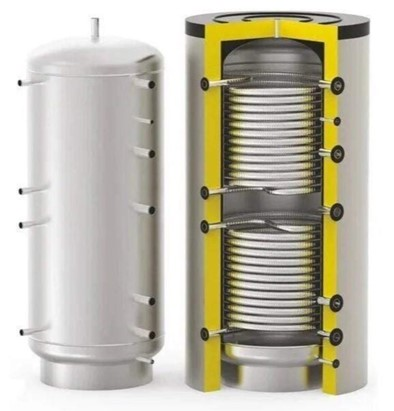
\includegraphics[width=6 cm]{images/water_tank_condenser.jpg}
    \caption{Water Tank with Two Condensing Coils [63]}
\end{figure}

\subsection{Electronic Expansion Valve Selection}

Selection of electronic expansion valves (EXV) is based on the following criteria:

\medskip
\begin{enumerate}[itemsep=3mm, parsep=-1mm, label=\roman*.]
    \item Suitable for HFC refrigerants (i.e., R-410A).
    \item Rated Capacity (kW).
\end{enumerate}

\medskip
Firstly, the selected valve must be compatible with the chosen refrigerant (i.e., R-410A).

\medskip
Secondly, the expansion valve must be able to provide the needed pressure reduction for system parameters. This is usually given by a vendor through an EXV’s capacity rating, which references the system’s heat removal rate in kW. Vendors provide a capacity rating for the following refrigerant conditions, based on AHRI standards [64]:

\medskip
\begin{table}[H]
\centering
\caption{AHRI Standard Rating Conditions for EXV}
\rowcolors{2}{gray!20}{white}
\begin{tabular}{|P{27mm}|P{35mm}|P{40mm}|P{40mm}|}
    \hline
    \rowcolor{orangeRed}
    Standard Rating Condition & Liquid Temperature at EXV Inlet & Condensing Temperature at EXV Inlet & Evaporating Temperature at EXV Outlet \\
    \hline
    A & 37\textdegree C & 38\textdegree C & 4\textdegree C \\
    \hline
\end{tabular}
\end{table}

\medskip
If the above standard is not used, vendors must specify the operating conditions used instead for their stated rating.

\medskip
Since these operating conditions differ from the ones in the DX-SAHP, a correction factor must be added to the required capacity rating, to compare it with ratings from the vendor. The following information is needed to determine the correction factor:

\medskip
\begin{enumerate}[itemsep=3mm, parsep=-1mm, label=\roman*.]
	\item Refrigerant: R-410A.
	\item Condenser capacity: $Q_L = 2.5 kW$.
	\item Evaporating temperature: $T_{evap} = \SI{-10}{\celsius}$.
	\item Condenser temperature: $T_{cond} = \SI{60}{\celsius}$.
	\item Subcooling: Assume subcooling of $\Delta T_{sub} = 4K$ at inlet of EXV.
\end{enumerate}

\medskip
All vendors include data sheets that specify the correction factors that must be used for their valve selection. The chosen valve was from manufacturer Danfoss who provided the following table [65] to aid in correction factor selection.

\medskip
\begin{table}[H]
\centering
\caption{Correction Factors for R-410A based on Degree of Subcooling}
\begin{tabular}{|P{35mm}|P{15mm}|P{15mm}|P{15mm}|P{15mm}|P{15mm}|}
    \hline
    \cellcolor{orangeRed}$\Delta T_{sub}$ & 0K & 4K & 10K & 15K & 20K \\
    \hline
    \cellcolor{orangeRed}Correction Factor & 1.00 & 1.06 & 1.14 & 1.21 & 1.28 \\
    \hline
\end{tabular}
\end{table}

\medskip
From Table 3.5, it can be seen that a correction factor of 1.06 must be used on $Q_L$ to get the nominal rating.
\begin{align}
    COP_{corrected} = \ddfrac{2.5kW}{1.06} = 2.36kW
\end{align}

\medskip
Thus $COP_{corrected}$ can be compared with ratings provided by the vendor at the system’s $T_{evap}$ and $T_{cond}$, to find to find an appropriate expansion valve.

\medskip
From this process it was found that the Danfoss ETS 6-10 [65] satisfied the needed capacity with a sufficient safety factor, being able to provide a capacity of $2.9 kW$ at the specified $T_{evap}$ and $T_{cond}$. For a full list of the vendor data sheets that were considered during EXV selection, please see the Electronic Expansion Valve selection document in the Design Binder.

\subsection{Piping}

Piping is an essential part of a heat pump; it carries the energy gained by the collector and compressor to be released in the condenser. A preliminary analysis was done to determine the drop in pressure between major components in the system. This pressure drop was considered to be from friction in the pipe, elbows, and changes in height. The variable definitions for all the equations below can be found in Appendix A.

\medskip
The equation for pressure drop due to friction in a circular pipe is given as [66]:
\begin{align}
    \Delta P_f = \ddfrac{fL_p \rho w^2}{2D_i}
\end{align}

\medskip
The friction factor, f, is calculated separately for laminar and turbulent flows; however, in this system, only turbulent flows were found. For turbulent flow, the Colebrook White equation [66] was used to calculate the friction factor. This was solved by moving all terms to one side and using the \verb|fzero| MATLAB [35] function to iteratively solve for the friction factor.
\begin{align}
    \frac{1}{\sqrt{f}} = -2.0log\left( \ddfrac{\frac{e}{D_i}}{3.7} + \frac{2.51}{Re\sqrt{f}}\right) 
\end{align}

The Reynold’s number determines the type of flow (i.e., Laminar, turbulent, or transitioning). If greater than 2320, the flow was considered turbulent. The Reynold’s Number was calculated as [66]:
\begin{align}
    Re = \ddfrac{wD_i}{\nu} = \ddfrac{\rho w D_i}{\mu}
\end{align}

\medskip
The values of density and viscosity were found using MATLAB to access CoolProp [18]. By specifying two state parameters, temperature and quality, the density and viscosity were obtained.

\medskip
The velocity of the refrigerant was calculated as:
\begin{align}
    w = \ddfrac{\dot m}{\frac{\rho \pi D_i^2}{4}}
\end{align}

\medskip
The pipe length between sections was assumed to be one meter for these calculations. Therefore, the pressure drop is shown per meter.

\medskip
The pressure drops were found for each section as described below:

\medskip
\begin{enumerate}[itemsep=3mm, parsep=-1mm, label= S\arabic*:]
	\item Between 1 (Compressor) and 2 (Condenser Inlet).
    \item Between 2 (Condenser Exit) and 3 (Expansion Valve).
    \item Between 3 (Expansion valve) and 4 (Evaporator Inlet).
    \item Between 4 (Evaporator Exit) and 1 (Compressor).
\end{enumerate}

\newpage
\begin{figure}[H]
    \centering
    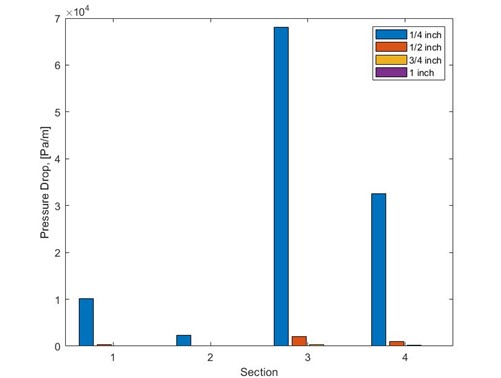
\includegraphics[width=11cm]{images/pressure_drops.jpg}
    \caption{Pressure Drop for \nicefrac{1}{4}, \nicefrac{1}{2}, \nicefrac{3}{4}, and 1 inch Diameter Piping at each Section}
\end{figure}

\medskip
As seen from Figure 3.10 above, the pressure drop in the \nicefrac{1}{4} inch pipe is magnitudes greater than it is for the other diameters. Figure 3.11 below shows the pressure drops for the \nicefrac{1}{2}, \nicefrac{3}{4}, and 1-inch diameters.

\medskip
\begin{figure}[H]
    \centering
    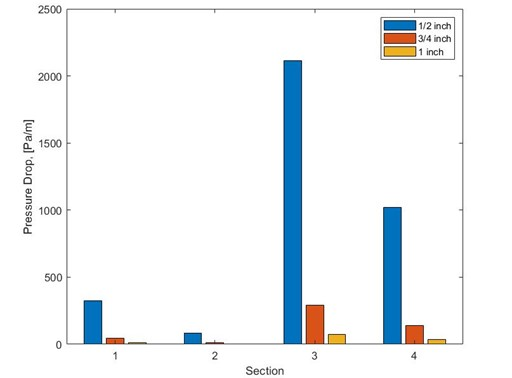
\includegraphics[width=11cm]{images/pressure_drops_new.jpg}
    \caption{Pressure Drop for \nicefrac{1}{2}, \nicefrac{3}{4}, and 1 inch Diameter Piping at each Section}
\end{figure}

\medskip
As seen from Figures 3.10 \& 3.11 above, as the diameter of the piping decreased, the pressure drop per meter increased drastically. Based on these values however, the pressure drop due to friction for diameters greater than \nicefrac{1}{4}” is insignificant considering the system operating pressures that range from $750kPa$ – $3800kPa$.

\medskip
The pressure drop due to elbows was calculated as follows [66]:
\begin{align}
    \Delta P_e = \ddfrac{K_L \rho w^2}{2}
\end{align}

\medskip
$K_L$ is the loss coefficient of the specified component or elbow. The loss coefficient for a long radius 90\textdegree \ flanged elbow is 0.2 and the loss coefficient for a regular 90\textdegree \ threaded elbow is 1.5 [66].

\medskip
The pressure drop due to a change in height was calculated as [66]:
\begin{align}
    \Delta P = \rho g \Delta z
\end{align}

\medskip
Since the piping is not yet finalized, the pressure drop due to elbows are shown for one elbow for each section.

\medskip
\begin{figure}[H]
    \centering
    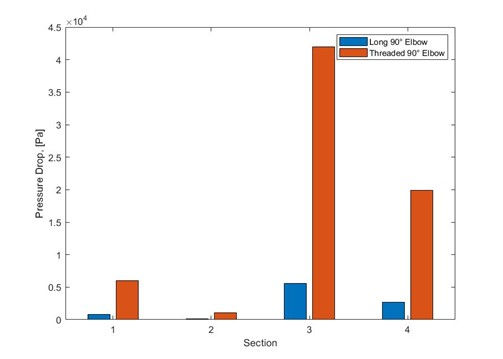
\includegraphics[width=11cm]{images/pressure_drops_elbows1.jpg}
    \caption{Pressure Drop from a Long Radius 90\textdegree \ Elbow vs. a Threaded 90\textdegree \ Elbow for a \nicefrac{1}{4} inch Pipe}
\end{figure}
\begin{figure}[H]
    \centering
    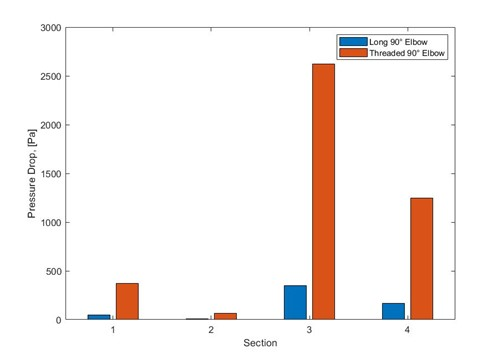
\includegraphics[width=11cm]{images/pressure_drops_elbows2.jpg}
    \caption{Pressure Drop from a Long Radius 90\textdegree \ Elbow vs. a Threaded 90\textdegree \ Elbow for a \nicefrac{1}{2} inch Pipe}
\end{figure}
\begin{figure}[H]
    \centering
    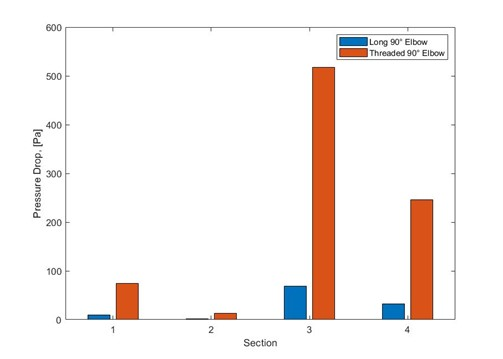
\includegraphics[width=11cm]{images/pressure_drops_elbows3.jpg}
    \caption{Pressure Drop from a Long Radius 90\textdegree \ Elbow vs. a Threaded 90\textdegree \ Elbow for a \nicefrac{3}{4} inch Pipe}
\end{figure}
\begin{figure}[H]
    \centering
    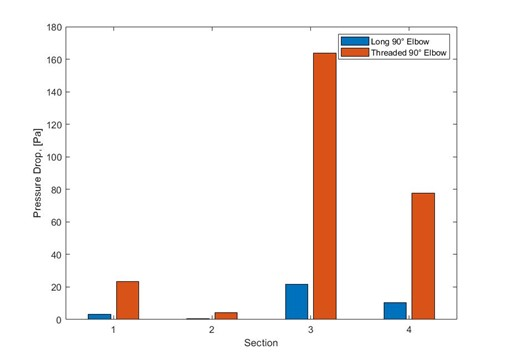
\includegraphics[width=11cm]{images/pressure_drops_elbows4.jpg}
    \caption{Pressure Drop from a Long Radius 90\textdegree \ Elbow vs. a Threaded 90\textdegree \ Elbow for a 1 inch Pipe}
\end{figure}

\medskip
As seen from Figures 3.12 - 3.15 above, the drop in pressure follows the same trend when decreasing the pipe diameter; smaller diameter has larger pressure drops. Additionally, the threaded 90\textdegree \ elbow yields more drop in pressure than the pipe with a large radius elbow as expected.

\medskip
Based on Figures 3.12 - 3.15, using a \nicefrac{1}{4}" copper pipe would result in too much pressure drop in our system; up to a max of $68kPa$ per meter and $19kPa$ per elbow. The \nicefrac{1}{2}" piping was found to have max pressure drops of $2.1kPa$ per meter and $2.6kPa$ per elbow. When considering installing the system for an average home, this may be too much loss in pressure. When comparing the \nicefrac{3}{4}” and 1” piping, both of their pressure drops are insignificant. For \nicefrac{3}{4}”, the max pressure drop was $0.29kPa$ per meter and $0.52kPa$ per elbow. For the 1” pipe, the max pressure drop was $0.071kPa$ per meter and $0.16kPa$ per elbow. To be more cost efficient, a piping size of \nicefrac{3}{4}” was found to be acceptable in minimizing pressure drop and cost.

\subsection{Minor Components}

\subsubsection{Accumulator}

A suction line accumulator is used to prevent any liquid from entering the compressor. If all the refrigerant exiting the collector is not vaporized, there is potential for liquid refrigerant to enter the compressor. Since this system uses a vapor compressor, any liquid refrigerant entering it will damage it. Additionally, the compressor is not modular, and any damage will require a full replacement, so protecting it is a necessity. An accumulator works by using a U-tube to trap any liquid refrigerant and only allowing vapor to flow to the compressor. The accumulator must be able to contain approximately seventy percent of the total refrigerant charge [67]. Additionally, during normal compressor operation, a small amount of oil from the compressor’s components will enter the piping; the accumulator also serves the purpose of collecting and returning this oil back to the compressor. To prevent any vapor from reaching the compressor, the accumulator is installed before the compressor [68].

\medskip
\begin{figure}[H]
    \centering
    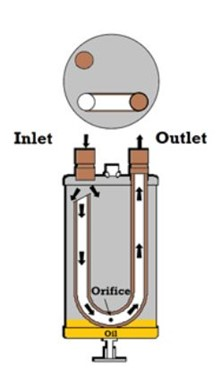
\includegraphics[width=3.5cm]{images/accumulator.jpg}
    \caption{Suction Line Accumulator [69]}
\end{figure}

\subsubsection{Filter Drier}

To keep the system working at optimal conditions, it is necessary to ensure that there are as little contaminants as possible. The potential contaminants in this system are water, copper shavings, or other contaminants during installation. The filter drier ensures these contaminants are not circulated throughout the system and causing damage; it is installed in the liquid-line of the heat pump before the sight glass [70].

\subsubsection{Sight Glass}

The sight glass is needed to view the level of the refrigerant to ensure proper operation. If there are bubbles seen through the sight glass it indicates that there is not enough refrigerant in the system. Additionally, the refrigerant must be subcooled before entering the EXV; therefore, the sight glass is installed before the EXV to ensure only liquid enters it [71].

\section{Control System}

The philosophy of having a control system for this design lies in the fact that the heat pump needs to adapt to varying ambient conditions to still meet the desired heat load. For instance, when there is less available sunlight, the pump might need to be active for a longer amount of time, simply due to the lower heat input rate.

\medskip
To ensure the heat load requirements are constantly being met, the system must control the following two parameters:

\medskip
\begin{enumerate}[itemsep=3mm, parsep=-1mm, label=\roman*.]
	\item Mass flow rate of the refrigerant.
	\item RPM of the compressor.
\end{enumerate}

\subsection{Mass Flow Rate Control}

Firstly, the mass flow rate of the refrigerant dictates how fast the refrigerant is flowing through the system. It is critical that the refrigerant enters the compressor as at least a saturated vapor, as any liquid-vapor mixture will damage the compressor. To ensure that full saturation is achieved, the refrigerant must spend enough time in the solar collector that it is able to fully change phase. The time spent in the collector is directly linked to mass flow rate and thus it is critical that this parameter be controlled. For example, during colder conditions where there is less available sunlight, the system needs to be able to lower the flow rate so that the refrigerant can spend more time in the collector to completely changing phase.

\medskip
Mass flow rate will be controlled by the electronic expansion valve. There is a stepper motor in the valve that incrementally opens and closes the valve opening, to adjust the flow rate. This stepper motor responds to electronic signals that will be fed by an external controller. The Danfoss controller [72] was selected as it is compatible with the system’s chosen electronic expansion valve. The controller input parameters include the refrigerant type, and the solar collector exit temperature and pressure. The temperature and pressure measurements will be given by an AKS model temperature sensor and an AKS 32R pressure transmitter, which are recommended from the controller’s operator’s manual [72]. The controller must optimize between ensuring that the refrigerant is at least a saturated vapor as it exits the collector, while still reducing the amount of superheat if possible. This is because excessive superheating at the outlet of the collector is an indicator that there is not enough refrigerant passing through and the mass flow rate should be increased. If the mass flow rate is needlessly low, the collector plate average temperature will increase, and $COP$ of the system will fall.

\begin{figure}[H]
    \centering
    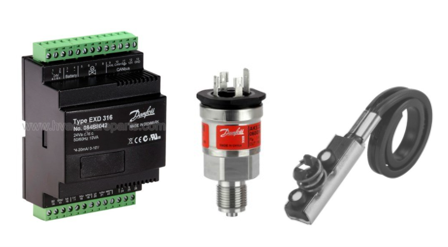
\includegraphics[width=8cm]{images/control_sensors.png}
    \caption{EXV Controller with Compatible Temperature and Pressure Sensors}
\end{figure}

\subsection{Compressor RPM Control}

Secondly, the RPM of the compressor must also be controlled. The RPM directly correlates to the pressure differential created by the compressor. To meet the heat load, the refrigerant conditions at the compressor outlet are taken to be constant at $331K$ and $3670 kPa$. The inlet conditions will be changing however depending on the evaporating temperature reached in the collector. This evaporating temperature is dictated by ambient conditions, and this leads to a situation where there are varying conditions at the inlet of the compressor and just a single outlet condition. Therefore, the compressor must change speed, depending on the inlet conditions, to create whatever pressure differential that is needed to get the refrigerant to the predefined outlet condition. Variable speed compressors are fitted with a temperature sensor at the inlet to determine refrigerant conditions. The needed outlet temperature can be set, and the controller within the compressor will adjust RPM accordingly.